\documentclass[problem]{mcs}

\begin{pcomments}
    \pcomment{TP_Spanning_Trees}
    \pcomment{Converted from prob4.scm
              by scmtotex and dmj
              on Sun 13 Jun 2010 11:22:25 AM EDT}
\end{pcomments}

\begin{problem}

%% type: short-answer
%% title: Spanning Trees

Find a spanning tree for the following graph by removing edges.
\begin{center}  
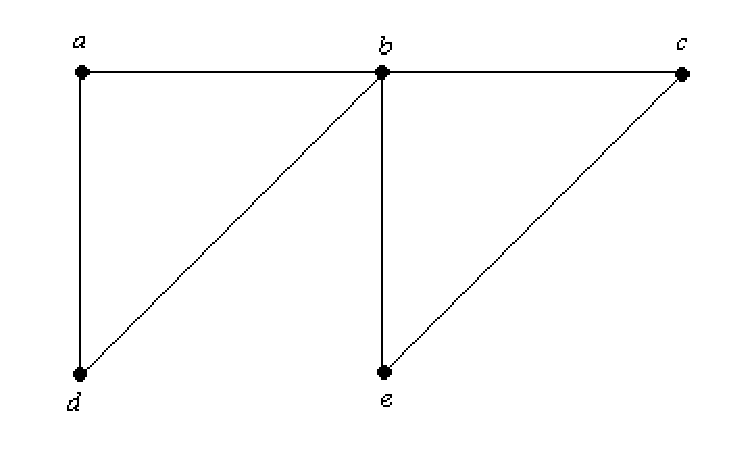
\includegraphics{pp5prob4}
\end{center}

%%  Type in the box the edges you remove.
%%  
%%  For each edge, you have to write the first letter in the pair first.
%%  
%%  For instance, you should write (a b) and not (b a).
%%  
%%  You should enter the edges separated by spaces: for example, if you
%%  want to answer (g k) and (u w), you should type
%%  
%%  \begin{equation*}
%%  (g k) (u w)
%%  \end{equation*}
%%  
%%  The order in which you enter the edges does not matter.

\begin{solution}

(a b), 
(b c)

(a b), 
(c e)

(a b), 
(b e)

(a d), 
(b c)

(a d), 
(c e)

(a d), 
(b e)

(b d), 
(b c)

(b d), 
(c e)

(b d), 
(b e)

Since the graph is connected, to make it a tree we need to break all
cycles.  There are only two cycles, and removing one edge from each is
enough to break them.
\end{solution}

\end{problem}

\endinput
